\section{Literature Review}
\label{sec:related_work}

\subsection{SimCLR: Simple Framework for Contrastive Learning of Visual Representations}

SimCLR\cite{chen2020simple} is a contrastive self-supervised learning framework that learns visual representations of images without requiring labeled data. The paper explores various components of the model and showcases the importance of each component via numbers from experiments.

The first key component of the SimCLR model is the augmentations it applies that leads to the positive and negative pairs needed to perform contrastive learning. The mentioned model stochastically chooses two augmentations from the chosen three augmentations to get the training pairs. The paper also mentions various other augmentations but reinforces the choice of the three augmentations (random crop, random colorization, and random Gaussian noise).

\begin{figure}[h]
\small
    \centering
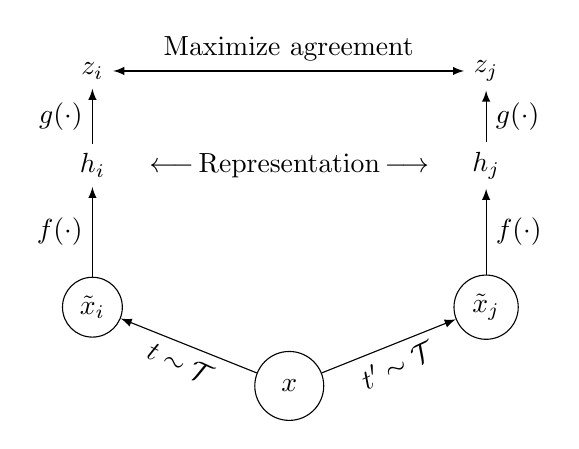
\begin{tikzpicture}
    \node at (0,1.8) (h) {$\longleftarrow\,$Representation$\,\longrightarrow$};
    \node[draw, circle] at (0,-1) (x) {$\,~\bm{x}~\,$};
    \node[draw, circle] at (-2.5,0) (x1) {$\tilde{\bm{x}}_i$};
    \node[draw, circle] at (2.5,0) (x2) {$\tilde{\bm{x}}_j$};
    \node at (-2.5,1.8) (h) {$\bm h_i$};
    \node at (2.5,1.8) (c) {$\bm h_j$};
    \node at (-2.5,3) (hh) {$\bm z_i$};
    \node at (2.5,3) (cc) {$\bm z_j$};
    \path[->] 
        (x)  edge [>=latex] node[below,rotate=-25] {$t\sim\mathcal{T}$} (x1)
        (x)  edge [>=latex] node[below,rotate=25] {$t'\sim \mathcal{T}$} (x2)
        (x1)  edge [>=latex] node[left,rotate=0] {$f(\cdot)$} (h)
        (x2)  edge [>=latex] node[right,rotate=0] {$f(\cdot)$} (c)
        (h)  edge [>=latex] node[left,rotate=0] {$g(\cdot)$} (hh)
        (c)  edge [>=latex] node[right,rotate=0] {$g(\cdot)$} (cc);
    \path[<->]
        (hh)  edge [>=latex] node[above,rotate=0] {Maximize agreement} (cc);
    \end{tikzpicture}
    \caption{A simple framework for contrastive learning of visual representations. 
    Two separate data augmentation operators are sampled from the same family of augmentations ($t\sim \mathcal{T}$ and $t'\sim \mathcal{T}$) and applied to each data example to obtain two correlated views.
    A base encoder network $f(\cdot)$ and a projection head $g(\cdot)$ are trained to maximize agreement using a contrastive loss. After training is completed, we throw away the projection head $g(\cdot)$ and use encoder $f(\cdot)$ and representation $\bm h$ for downstream tasks.}
    \label{fig:framework}
\end{figure}

Batches of such augmented images are fed to the encoder component where a ResNet architecture was used. The paper then experimented with different projection layers and showed via experimentation that a non-linear projection component worked the best. The contrastive loss is then applied to these projected outputs. SimCLR shows various key components that can be used to extract representations in a self-supervised manner which can be made use of to come up with an explainable self-supervised learning model.

\subsection{Grad-CAM: Visual Explanations from Deep Networks via Gradient-based Localization (Selvaraju et al., ICCV 2017)}

Gradient-weighted Class Activation Mapping (Grad-CAM)\cite{Selvaraju_2017_ICCV} is a widely adopted method that provides visual explanations for model predictions by leveraging gradient information to highlight the most important regions in an input image. Unlike earlier Class Activation Mapping (CAM) approaches, which required model modifications, Grad-CAM is architecture-agnostic and can be applied to various types of model architectures.

Grad-CAM generates class-specific saliency maps by computing the importance of feature maps in a CNN for a given target class. The method consists of the following steps:

1. \textbf{Forward Pass:} The input image is processed through the CNN, and feature maps \(A^k\) from a selected convolutional layer are extracted.

2. \textbf{Gradient Computation:} The gradients of the target class score \(y^c\) are computed with respect to each feature map:

   $$
   \alpha_k^c = \frac{1}{Z} \sum_i \sum_j \frac{\partial y^c}{\partial A^k_{ij}}
   $$

   where \(Z\) represents the spatial dimensions of the feature map.

3. \textbf{Weighted Feature Map Combination:} A weighted sum of the feature maps is computed using the importance weights \(\alpha_k^c\):

   $$
   L_c = \text{ReLU} \left( \sum_k \alpha_k^c A^k \right)
   $$

   The ReLU function ensures that only positive influences contribute to the visualization, preventing the inclusion of irrelevant or misleading features.

4. \textbf{Heatmap Generation and Overlay:} The resulting saliency map is re-sampled to the original image resolution and overlayed on the input image to highlight the key regions that contribute to the model decision.

\begin{figure}[h]
    \centering
    \includegraphics[width=0.47\textwidth]{./images/Grad-CAM_approach.png}
    \caption{Grad-CAM visualization of a ResNet-50 model for the class "zebra." The heatmap highlights the regions in the input image that are most relevant for the model's prediction.}
    \label{fig:gradcam}
\end{figure}


Although Grad-CAM is highly effective in supervised learning scenarios, its applicability to self-supervised learning (SSL) models presents significant challenges. SSL approaches, such as SimCLR and MoCo, do not rely on explicit class labels, making the traditional Grad-CAM formulation which depends on class scores for gradient computation. To overcome these challenges, we propose several modifications to adapt Grad-CAM for self-supervised learning:

1. \textbf{Using Contrastive Loss Gradients:} Instead of computing gradients with respect to class scores, we leverage gradients from the contrastive loss function (e.g., InfoNCE loss). This allows us to identify which regions of an image contribute the most to effective representation learning.

2. \textbf{Feature Importance Analysis at Intermediate Layers:} Since SSL models do not use final classification layers, Grad-CAM can be applied to intermediate feature representations before projection layers to understand which regions are most influential in encoding meaningful representations.

3. \textbf{Downstream Evaluation via Linear Probing:} To bridge SSL and interpretability, a linear classifier can be trained on SSL embeddings for a downstream task (e.g., object classification). Grad-CAM can then be used to visualize how well SSL representations capture class-discriminative features.

\subsection{RELAX: Representation Learning Explainability}
\begin{itemize}
    \item Representation Learning Explainability (RELAX)\cite{wickstrøm2022relaxrepresentationlearningexplainability} is a novel framework for explaining representations that also quantify their uncertainty.
    \item It measures the change in the representation of an image when compared with the masked version of the image.
    \item The central idea is that when informative parts are masked out, the representation should change significantly, i.e., the similarity between masked and unmasked representations should be low when informative parts are masked out and high when uninformative parts are masked out.
\end{itemize} 
Let $\mathbf{X}\in \mathbb{R}^{H\times W}$ represents image of dimensions $H\times W$ and $f$ be the feature extraction model that extracts representation $\mathbf{h} = f(\mathbf{X}) \in \mathbb{R}^D$. \\
To create masked images, we apply a stochastic mask $\mathbf{M}\in [0, 1]^{H\times W}$, where $M_{ij}$ is drawn from some distribution.
The masked representation is given by $\bar{\mathbf{h}} = f(\mathbf{X}\odot \mathbf{M})$, where $\odot$ denotes element-wise multiplication.\\
The similarity between masked and unmasked representations is measured using cosine similarity, 
\begin{equation*}\label{eq:sim}
    s(\mathbf{h}, \bar{\mathbf{h}}) = \frac{\langle \mathbf{h}, \bar{\mathbf{h}}\rangle }{\lVert\mathbf{h}\rVert \lVert\bar{\mathbf{h}}\rVert},
\end{equation*}, where $\lVert\cdot\rVert$ denotes the Euclidean norm of a vector. \\
Importance $R_{ij}$ of pixel $(i,j)$ is defined as:
\begin{equation*}\label{eq:rel1}
    R_{ij} = \mathrm{E}_{\mathbf{M}}\big[s(\mathbf{h}, \bar{\mathbf{h}})M_{ij}\big].
\end{equation*}
\begin{equation*}\label{eq:rel2}
    \bar{R}_{ij} = \frac{1}{N}\sum\limits_{n=1}^N s(\mathbf{h}, \bar{\mathbf{h}}_n)M_{ij}(n).
\end{equation*}
The uncertainty $U_{ij}$ of pixel $(i,j)$ is defined as:
\begin{equation*}\label{eq:unc1}
    U_{ij} = \mathrm{Var}_{\mathbf{M}} [s(\mathbf{h}, \bar{\mathbf{h}})M_{ij}].
\end{equation*}
\begin{equation*}\label{eq:unc2}
    \bar{U}_{ij} = \frac{1}{N}\sum\limits_{n=1}^N (s(\mathbf{h}, \bar{\mathbf{h}}_n) - \bar{R}_{ij})^2 M_{ij}(n).
\end{equation*}

The figure \ref{fig:relax}, shows an example where RELAX is used to investigate the explanations and uncertainities for a selection of widely used feature extraction models. Red indicates high values, and blue indicates low values. In the figure, two birds are present, one prominently displayed in the foreground and another in the background. The plot shows all models emphasize the bird in the foreground with low uncertainty. However, the emphasis on the bird in the background varies with different degrees of uncertainty. 
\begin{figure}[h]
    \centering
    \includegraphics[width=0.47\textwidth]{./images/VOCexample.pdf}
    \caption{RELAX explations and uncertainty estimates for a VOC image.}
    \label{fig:relax}
\end{figure}

\subsection{Prototypical Networks for Unsupervised Disentanglement}
ProtoVAE is a novel Variational Autoencoder (VAE)-based framework\cite{patil2023protovaeprototypicalnetworksunsupervised} that incorporates Prototypical Networks to enforce structured disentanglement of latent representations in a completely self-supervised manner. The model achieves this by applying interventions in latent space, where a single latent dimension is modified while keeping others unchanged. The VAE acts as the generative component, while the Prototypical Network clusters latent representations, ensuring that each dimension encodes a distinct and interpretable factor of variation. A local isometry constraint is introduced to maintain smooth and meaningful changes in data space when traversing latent dimensions. Additionally, a discriminator network regularizes the latent space, ensuring that modified representations still map to valid data distributions. Empirical results demonstrate state-of-the-art disentanglement on benchmark datasets such as dSprites, 3DShapes, MPI3D, and CelebA.

In our project, we aim to improve interpretability in Self-Supervised Learning (SSL) representations, particularly for contrastive learning methods like SimCLR. We can leverage ProtoVAE’s self-supervised latent disentanglement framework to introduce structured clustering in SSL embeddings, making them more explainable. By integrating a Prototypical Network, we can group semantically similar representations, providing insights into how SSL learns features. Furthermore, the interventional approach used in ProtoVAE can be adapted to analyze individual feature importance in SSL embeddings. By combining this with Grad-CAM and concept-based methods, we can provide more transparent and interpretable explanations of SSL representations, bridging the gap between performance and trust in self-supervised models.
